\documentclass[letterpaper,10pt,oneside]{article}

\usepackage[style=authoryear, backend=biber, natbib=true]{biblatex}

\bibliography{mybib}

\usepackage{graphicx}
\graphicspath{ {/Users/jacksonwills/Documents/Fitz_Research/Report} }

\usepackage{amsmath, amssymb, amsfonts, bm, mathtools}
\usepackage{hyperref}


\title{System Modeling and Control of the Furuta Pendulum}
\author{Jackson Wills}



\begin{document}

\maketitle

\tableofcontents

\newpage

Random citation \cite{SWINGUP} embeddeed in \citet{SWINGUP} text \cite{DYNAMICS}

\section{System Decription}

In this paper, the dynamics of the Furuta Pendulum are simulated and the system is given reasonable parameters and controlled using linear full-state feedback control. The Furuta Pendulum was developed by a man named Katsuhisa Furuta at the Tokyo Institute of Technology in 1992. The device consists of an motor which can rotate a beam in the horizontal plane. Attatched to that beam is a pendulum which is free to rotate in the vertical plane - see figure \ref{fig:diagram}.


\begin{figure}[h!]
  % The [h!] puts the figure right here instead of at the top of the page, which is the default.
  \centering
  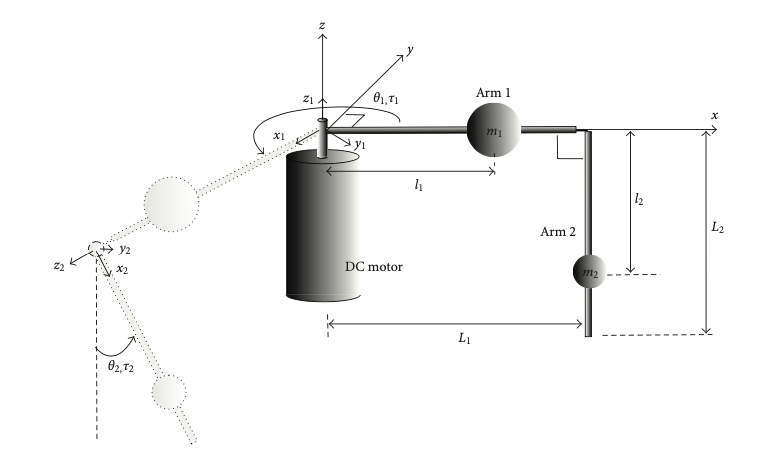
\includegraphics[width=0.9\textwidth]{FurutaDiagram}
  % This makes the diagram be .9 times the width of the text!
  \caption{A diagram of the Furuta Pendulum \citep{DYNAMICS}}
  \label{fig:diagram}
  % label is cool! This lets me refernce the figure, even when the figure number changes.
\end{figure}

\section{Derivation of the Equations of Motion}

The first thing to do is to get equations of motion which accurately model the system. These equations were derived largely with the help of \cite{DYNAMICS}. The equations of motion were found to be \\
% the citep puts parentesis around the name and date of the author. To get numberical citing, change the \usepackage{biblatex} options

% could also have used cite or citet



\begin{multline}
  0 = - 2.0 J_{2xx} \dot{\theta}_{1} \dot{\theta}_{2} \sin{\left(\theta_{2}{\left(t \right)} \right)} \cos{\left(\theta_{2}{\left(t \right)} \right)} + 2.0 J_{2yy} \dot{\theta}_{1} \dot{\theta}_{2} \sin{\left(\theta_{2}{\left(t \right)} \right)} \cos{\left(\theta_{2}{\left(t \right)} \right)}
        \\
   + 1.0 L_{1} l_{2} m_{2} \ddot{\theta}_{2} \cos{\left(\theta_{2}{\left(t \right)} \right)} - 1.0 L_{1} l_{2} m_{2} \dot{\theta}_{2}^{2} \sin{\left(\theta_{2}{\left(t \right)} \right)} + b_{1} \dot{\theta}_{1} + \\ 2.0 l_{2}^{2} m_{2} \dot{\theta}_{1} \dot{\theta}_{2} \sin{\left(\theta_{2}{\left(t \right)} \right)} \cos{\left(\theta_{2}{\left(t \right)} \right)} - \tau_{1}
    \\
    % It is important that the new line of the equation starts with an + or -
    + \ddot{\theta}_{1} \left[1.0 J1zz + 1.0 J_{2xx} \cos^{2}{\left(\theta_{2}{\left(t \right)} \right)} + 1.0 J_{2yy} \sin^{2}{\left(\theta_{2}{\left(t \right)} \right)} + 1.0 L_{1}^{2} m_{2} \sin^{2}{\left(\theta_{2}{\left(t \right)} \right)}
      \right.
      \\
      \left.
      % I put these left. and right. in there bacause the parentesis went over a line break that I wanted to make.      Note the periods after the left. and right.        Also, I made the parentesis that crossed the line into a braket to make it clearer. I don't think this is necessary and it may even be bad practice.
     + 1.0 L_{1}^{2} m_{2} \cos^{2}{\left(\theta_{2}{\left(t \right)} \right)} + 1.0 l_{1}^{2} m_{1} + 1.0 l_{2}^{2} m_{2} \sin^{2}{\left(\theta_{2}{\left(t \right)} \right)}\right]
\end{multline}
% I used multline to create a math enviornment, but thats only because the equations were so long. align is better for shorter things. The & symbol is where the two equations align themselves. Shown here is an unrelated example of align.
%\begin{align}
  %x &= \left( 2 + \frac{1}{3} \right) %\label{eq:important}\\
  %y &= 4x
%\end{align}
% Some random text. See \eqref{eq:important} for blah.
\begin{multline}
  0 = 1.0 J_{2zz} \ddot{\theta}_{2} + 1.0 L_{1} l_{2} m_{2} \ddot{\theta}_{1} \cos{\left(\theta_{2}{\left(t \right)} \right)} + b_{2} \dot{\theta}_{2} + g l_{2} m_{2} \sin{\left(\theta_{2}{\left(t \right)} \right)}
      \\
   + 1.0 l_{2}^{2} m_{2} \ddot{\theta}_{2} - \tau_{2} + \dot{\theta}_{1}^{2} \left[1.0 J_{2xx} \sin{\left(\theta_{2}{\left(t \right)} \right)} \cos{\left(\theta_{2}{\left(t \right)} \right)}
\right.
\\
\left.
   - 1.0 J_{2yy} \sin{\left(\theta_{2}{\left(t \right)} \right)} \cos{\left(\theta_{2}{\left(t \right)} \right)} - 1.0 l_{2}^{2} m_{2} \sin{\left(\theta_{2}{\left(t \right)} \right)} \cos{\left(\theta_{2}{\left(t \right)} \right)}\right]
\end{multline}

These equations were then linearized about $\theta_{1} = \pi$ and $\theta_{2} = 0.$ \\
The goal of the control law was to keep $\theta_{1}$ at  $\pi$, assuming the system started near $\pi$.\\

A linear full-state feedback control law was implemented and the resulting gain matrix is: \\

$ k =
\begin{bmatrix}
  8.53 &
  -15.90 &
  -3.66 &
  -0.97
\end{bmatrix}$

\begin{align}
  k = \left[\begin{array}{cccc}
  8.53 &
  -15.90 &
  -3.66 &
  -0.97
  \end{array}\right]
\end{align}


\section{New section}
\subsection{New Subsection}

\newpage




\newpage
\appendix
\section{EOM Derivation}
\label{EOM}

\section{Bibliography}
\printbibliography

\end{document}
